% Created 2026-07-09 qui 11:28
% Intended LaTeX compiler: lualatex
\documentclass[12pt,a4paper]{article}
\usepackage{fgv-paper}
\usepackage{longtable}
\usepackage{booktabs}
\usepackage{pdflscape}
\usepackage{array}
\usepackage[backend=biber,sorting=nty,giveninits=true]{biblatex}

\usepackage{graphicx}
\author{Gustavo M. Mendes de Tarso}
\date{2026}
\title{Redesenho do fluxo de análise dos benefícios por incapacidade na Perícia Médica Federal: revisão de evidências sobre triagem documental, teleperícia e alocação de capacidade}
\hypersetup{
 pdfauthor={Gustavo M. Mendes de Tarso},
 pdftitle={Redesenho do fluxo de análise dos benefícios por incapacidade na Perícia Médica Federal: revisão de evidências sobre triagem documental, teleperícia e alocação de capacidade},
 pdfkeywords={},
 pdfsubject={},
 pdfcreator={Emacs 28.2 (Org mode 9.5.5)}, 
 pdflang={Brazilian}}
\begin{document}

\maketitle
\tableofcontents


\section{Identificação}
\label{sec:org3a2ab8a}
\begin{itemize}
\item Perfil: \texttt{relatorio\_prisma\_busca\_orientada\_fgv}.
\item Etapa: consolidação após triagem humana.
\item Layout institucional: paper\textsubscript{fgv}.
\item Projeto: prisma\textsubscript{fluxo}\textsubscript{pmf}.
\end{itemize}

\section{Questão e escopo da revisão}
\label{sec:orgac75468}
\begin{itemize}
\item Tema: Redesenho baseado em evidências do fluxo de análise dos benefícios por incapacidade na Perícia Médica Federal
\item Recorte: Brasil; organização do fluxo entre análise documental, teleperícia, perícia presencial, capacidade ordinária e mutirões. O ATESTMED é tomado como referência institucional de análise documental, sem restringir a busca à experiência brasileira.
\item Objetivo: Analisar evidências e alternativas para redesenhar o tratamento de requerimentos por incapacidade, combinando análise documental, avaliação remota, perícia presencial, capacidade territorial e critérios auditáveis de alocação.
\item Pergunta de pesquisa: Como estruturar um fluxo de alocação de requerimentos entre análise documental, teleperícia e perícia presencial que reduza o tempo de espera sem comprometer a qualidade decisória, a equidade territorial e o controle?
\item Tipo de estudo: revisão estruturada de evidências para análise e redesenho de política pública
\end{itemize}

\section{Protocolo de busca}
\label{sec:orgeca513e}
\begin{itemize}
\item Estratégia: \texttt{blocos\_tematicos}.
\end{itemize}
\subsection{Blocos e consultas executadas}
\label{sec:org84c8a86}
\begin{itemize}
\item Benefícios por incapacidade e avaliação médico-pericial: \texttt{disability benefits AND medical assessment}
\item Benefícios por incapacidade e avaliação médico-pericial: \texttt{incapacity benefit AND medical evaluation}
\item Benefícios por incapacidade e avaliação médico-pericial: \texttt{work disability AND medical certification}
\item Análise documental e elegibilidade: \texttt{documentary assessment AND disability}
\item Análise documental e elegibilidade: \texttt{medical certificate AND disability benefits}
\item Análise documental e elegibilidade: \texttt{medical documentation AND work incapacity}
\item Teleperícia e avaliação remota: \texttt{remote medical assessment AND disability}
\item Teleperícia e avaliação remota: \texttt{telemedicine AND disability assessment}
\item Teleperícia e avaliação remota: \texttt{telehealth AND medical certification}
\item Capacidade, filas e alocação de serviços: \texttt{disability benefits AND waiting time}
\item Capacidade, filas e alocação de serviços: \texttt{medical assessment AND service capacity}
\item Capacidade, filas e alocação de serviços: \texttt{case allocation AND disability services}
\item Equidade territorial, qualidade e controle: \texttt{disability assessment AND equity of access}
\item Equidade territorial, qualidade e controle: \texttt{remote assessment AND quality assurance}
\item Equidade territorial, qualidade e controle: \texttt{medical certification AND audit}
\item Palavras-chave: benefícios por incapacidade; disability benefits assessment; análise documental de incapacidade; documentary review disability claims; teleperícia; telemedicine disability evaluation; perícia médica presencial; triagem de requerimentos por incapacidade; work capacity assessment; gestão de filas em saúde; equidade territorial no acesso; auditabilidade de decisões administrativas
\item Idiomas: português; inglês; espanhol
\item Bases selecionadas: Crossref; OpenAlex; Semantic Scholar; Scopus; Web of Science; PubMed/NCBI; Europe PMC; SciELO; CORE
\end{itemize}

\subsection{Critérios de inclusão}
\label{sec:orge3e4dc1}
\begin{itemize}
\item Estudos que analisem benefícios por incapacidade, afastamento por doença, seguro por incapacidade, certificação médica ou avaliação médico-pericial.
\item Estudos que abordem triagem documental, elegibilidade, análise de documentos médicos, validação de atestados ou processos de decisão sobre incapacidade.
\item Estudos que examinem teleperícia, telemedicina aplicada à avaliação, avaliação médica remota, videoperícia ou modalidades híbridas de avaliação.
\item Estudos que analisem capacidade operacional, filas, tempo de espera, produtividade, priorização de casos, alocação de profissionais ou gestão de demanda em serviços periciais ou sistemas de benefícios.
\item Estudos que discutam acesso territorial, equidade, barreiras geográficas, inclusão de populações remotas ou desigualdades de acesso à avaliação médico-pericial.
\item Estudos que tratem de qualidade decisória, confiabilidade, auditoria, controle, integridade, prevenção de fraude, revisão de decisões ou riscos associados à avaliação remota ou documental.
\item Estudos empíricos, avaliações de política pública, estudos de caso institucionais, revisões sistemáticas, revisões de escopo ou relatórios técnicos com evidência útil para a pergunta de pesquisa.
\item Publicações em português, inglês ou espanhol.
\end{itemize}

\subsection{Critérios de exclusão}
\label{sec:orge9375fa}
\begin{itemize}
\item Telemedicina exclusivamente assistencial, sem relação substantiva com avaliação de incapacidade, certificação, elegibilidade, triagem ou gestão de fluxos.
\item Estudos clínicos que não contribuam para compreender processos de avaliação médico-pericial, decisão administrativa, capacidade, acesso, qualidade ou controle.
\item Textos sem relação substantiva com a pergunta de pesquisa ou com ao menos um eixo da matriz analítica.
\item Editorial, comentário, notícia, apresentação, resumo de congresso ou opinião sem análise, dados, revisão ou contribuição institucional verificável.
\item Duplicidades entre bases ou consultas.
\item Registros sem título, resumo ou metadados suficientes para triagem humana.
\item Publicações em idioma diferente de português, inglês ou espanhol quando não houver informação suficiente para avaliação confiável.
\end{itemize}

\section{Registro por fonte}
\label{sec:orgf89172a}
\begin{center}
\begin{tabular}{lrl}
Base & Registros recuperados & Situação\\
\hline
Crossref & 300 & ok\\
OpenAlex & 300 & ok\\
Semantic Scholar & 200 & parcial\\
Scopus & 15 & ok\\
Web of Science & 0 & não executada: credencial ausente\\
PubMed/NCBI & 289 & ok\\
Europe PMC & 300 & ok\\
SciELO & 0 & bloqueada por anti-automação\\
CORE & 255 & parcial\\
\end{tabular}
\end{center}

\section{Fluxo de seleção}
\label{sec:org4fe151b}

\begin{figure}[htbp]
\centering
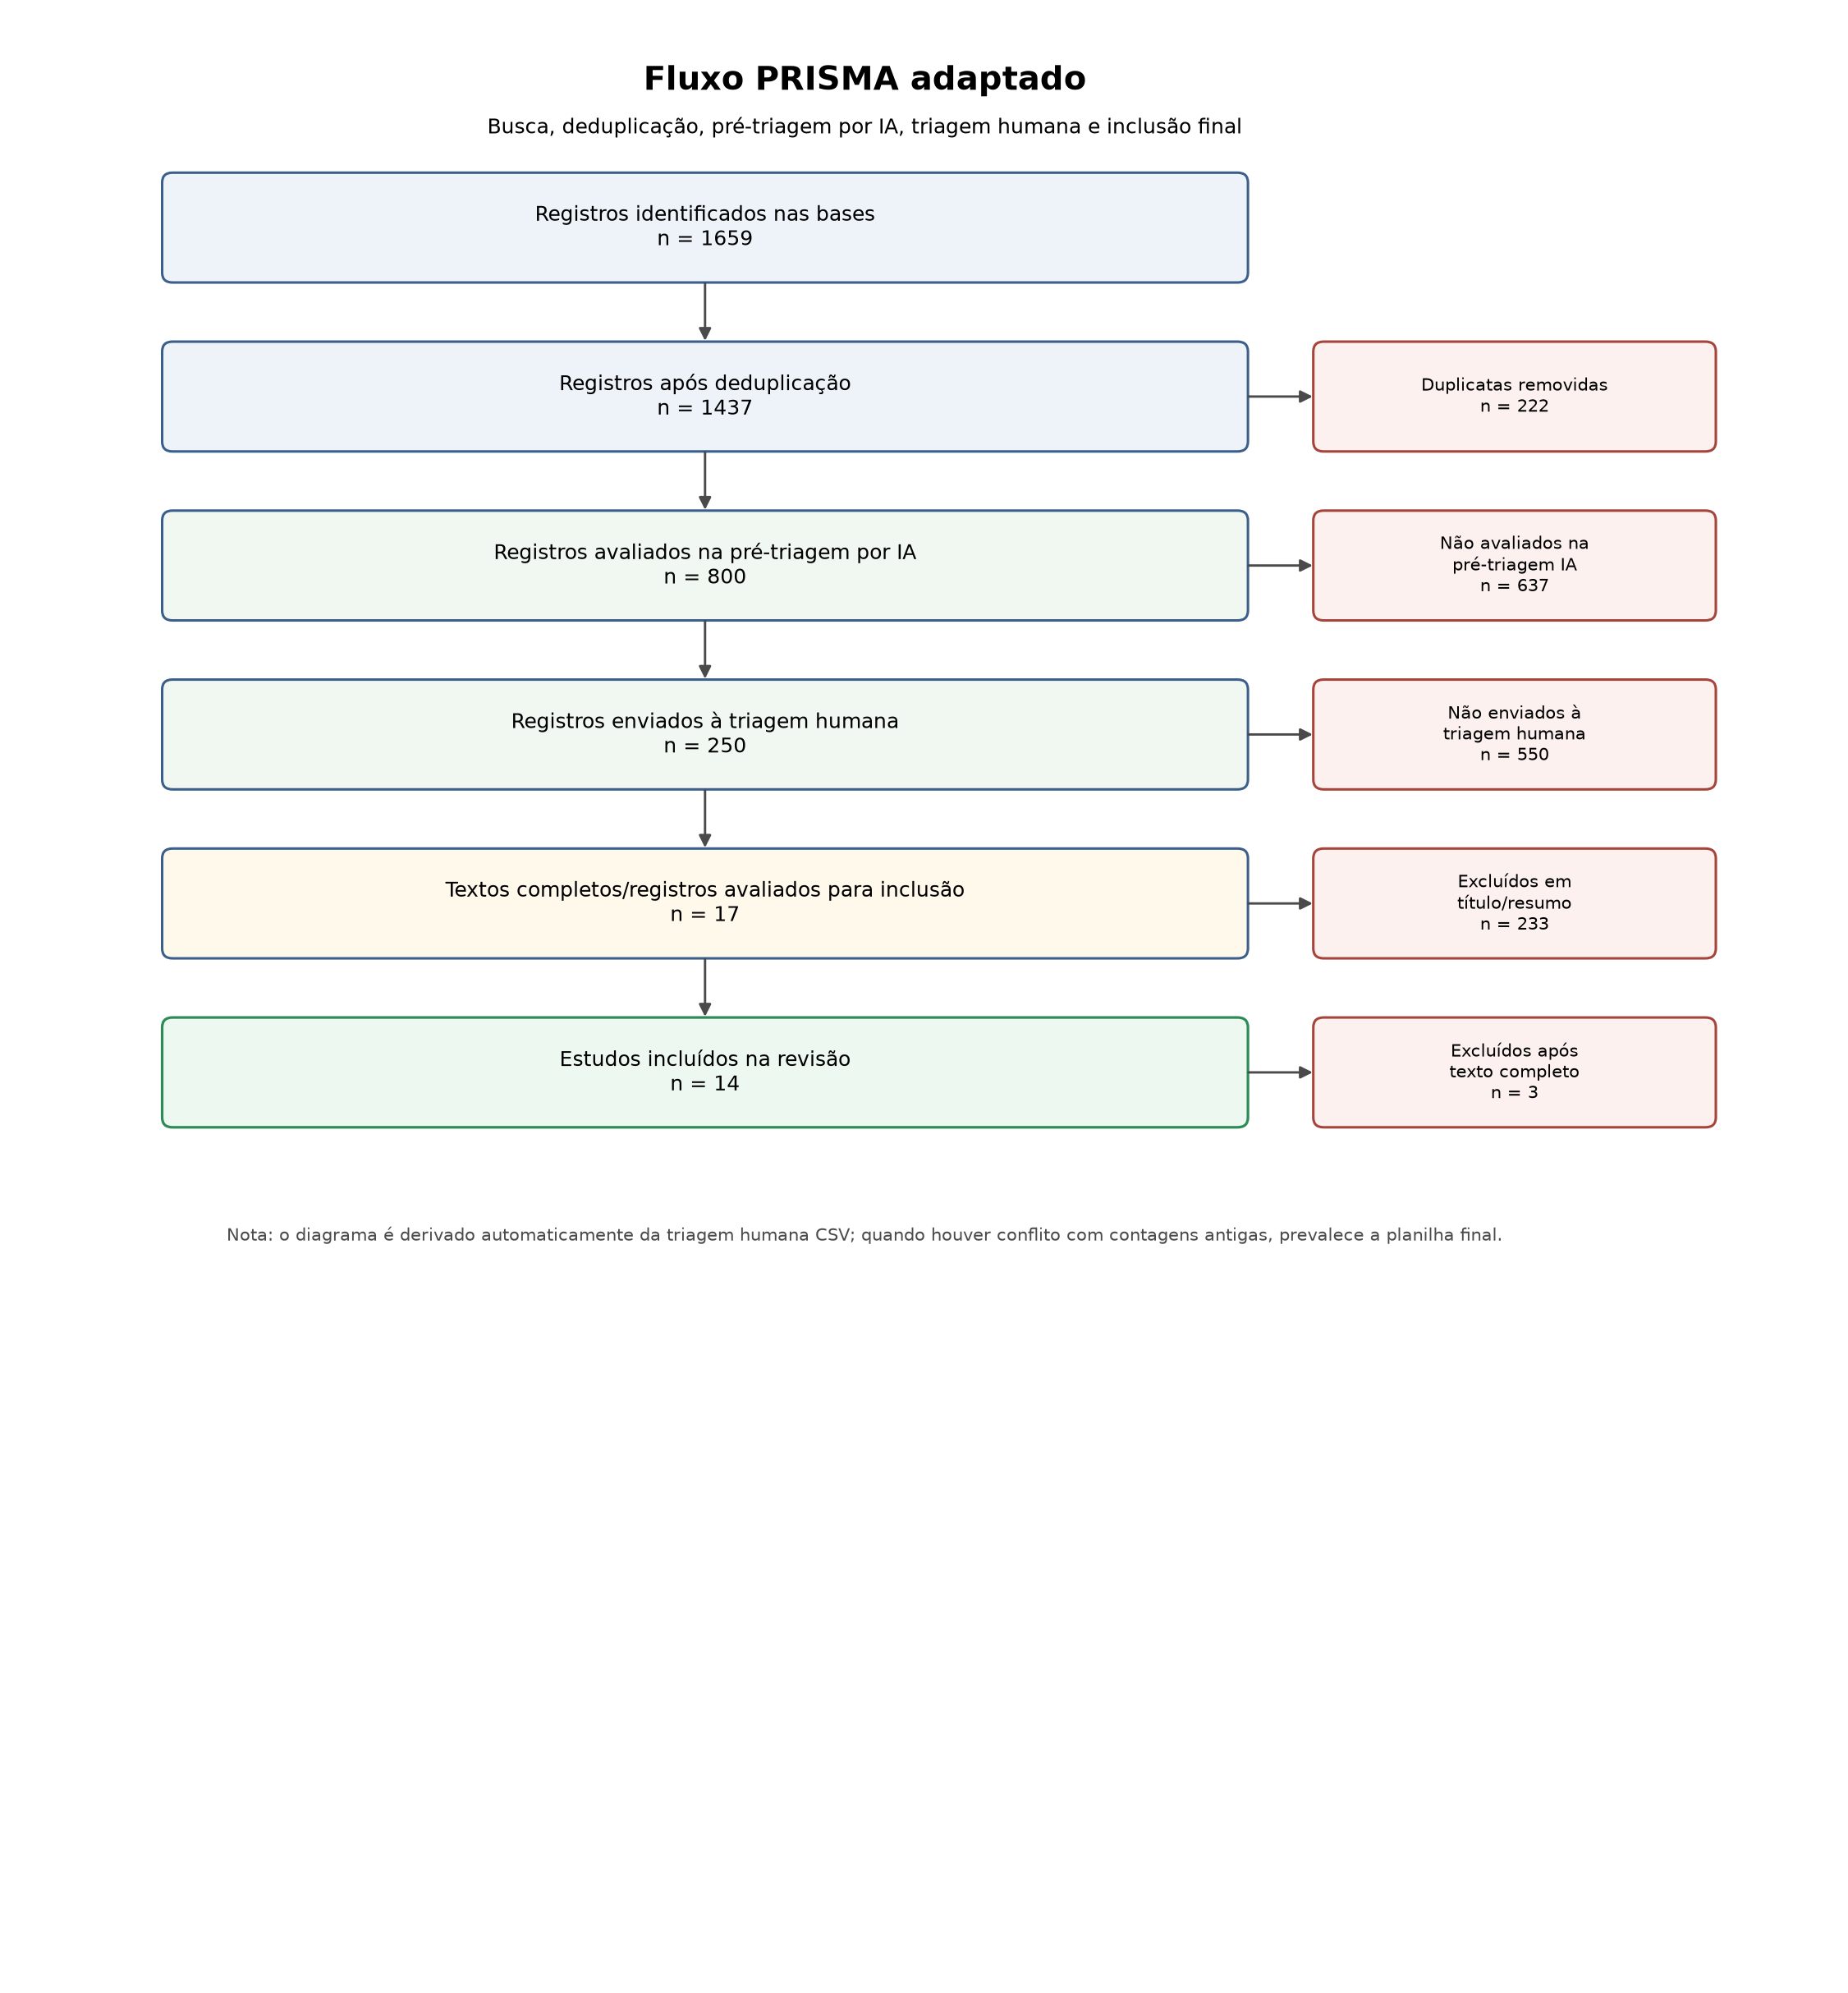
\includegraphics[width=0.95\textwidth]{relatorio_prisma_prisma_fluxo_pmf.diagrama_prisma.png}
\caption{Diagrama PRISMA adaptado ao fluxo de busca, pré-triagem por IA e triagem humana.}
\end{figure}

\begin{center}
\begin{tabular}{lr}
Etapa & Quantidade\\
\hline
registros identificados & 1659\\
duplicatas removidas & 222\\
registros apos deduplicacao & 1437\\
registros pre triagem ia avaliados & 800\\
registros enviados para triagem & 250\\
triagem titulo resumo concluida & 250\\
registros excluidos titulo resumo & 233\\
textos completos avaliados & 17\\
textos completos excluidos & 3\\
estudos incluidos & 14\\
registros na planilha & 250\\
\end{tabular}
\end{center}

A figura apresenta o funil de seleção da revisão. As contagens finais de triagem humana são derivadas do arquivo \texttt{triagem\_humana.csv}; quando contagens intermediárias antigas entram em conflito com a planilha final, prevalece a reconciliação pela decisão humana final.

\section{Estudos incluídos}
\label{sec:org6ef67f4}
\begin{enumerate}
\item N. Di Fazio; G. Delogu; D. Morena; Eugenia Carfora; Dalila Tripi; R. Rinaldi; P. Frati; V. Fineschi (2024). Telehealth Intervention: A Proposal for a Telemedicine Manual to Ascertain the Civil Disability Status in Italy. International Journal of Environmental Research and Public Health. DOI: \url{https://doi.org/10.3390/ijerph21030253}.
\item Geiger; Garthwaite; Warren; Bambra (2018). Assessing work disability for social security benefits: international models for the direct assessment of work capacity. Disability and Rehabilitation. DOI: \url{https://doi.org/10.1080/09638288.2017.1366556}.
\item Kim; Kim (2025). Medical certification in sickness benefit scheme (II): practical approaches for evaluating work disability. Annals of Occupational and Environmental Medicine. DOI: \url{https://doi.org/10.35371/aoem.2025.37.e24}.
\item Romy Steenbeek; Antonius JM Schellart; Henny Mulders; Johannes R. Anema; Herman Kroneman; Jan Besseling (2011). The development of instruments to measure the work disability assessment behaviour of insurance physicians. BMC Public Health. DOI: \url{https://doi.org/10.1186/1471-2458-11-1}.
\item Yangwoo Kim; Inah Kim (2025). Medical certification in sickness benefit schemes (I): theoretical perspectives and return-to-work. Annals of Occupational and Environmental Medicine. DOI: \url{https://doi.org/10.35371/aoem.2025.37.e23}.
\item Jessica Anner; Urban Schwegler; Regina Kunz; Bruno Trezzini; Wout de Boer (2012). Evaluation of work disability and the international classification of functioning, disability and health: what to expect and what not. BMC Public Health. DOI: \url{https://doi.org/10.1186/1471-2458-12-470}.
\item Vasudeva; Sheikh; Sahu (2021). International Classification of Functioning, Disability, and Health augmented by telemedicine and artificial intelligence for assessment of functional disability. Journal of Family Medicine and Primary Care. DOI: \url{https://doi.org/10.4103/jfmpc.jfmpc\_692\_21}.
\item T. Rosburg; R. Kunz; B. Trezzini; Urban Schwegler; J. Jeger (2021). The assessment of capacity limitations in psychiatric work disability evaluations by the social functioning scale Mini-ICF-APP. BMC Psychiatry. DOI: \url{https://doi.org/10.1186/s12888-021-03467-w}.
\item Riley Bove; Carolyn Bevan; Elizabeth Crabtree; Chao Zhao; Refujia Gomez; Priya Garcha; John Morrissey; Jason Dierkhising; Ari Green; Stephen L. Hauser; Bruce Cree; Mitchell T. Wallin; Jeffrey M. Gelfand (2018). Toward a low-cost, in-home, telemedicine-enabled assessment of disability in multiple sclerosis. Multiple Sclerosis Journal. DOI: \url{https://doi.org/10.1177/1352458518793527}.
\item Georgios Theotokatos; R. Escorpizo; T. Angelopoulos; Nikolaos Chrysagis; Jerome Bickenbach; Aikaterini Venieri; Konstantinos Karteroliotis; E. Grammatopoulou; E. Skordilis (2023). Psychometric Properties of the 12-Item World Health Organization Disability Assessment Schedule (WHODAS 2.0), Greek Version: A Cross-Sectional Study on Applicants of Welfare Benefits. Cureus. DOI: \url{https://doi.org/10.7759/cureus.48588}.
\item Guo; Togher; Power; Hutomo; Yang; Tay; Yen; Koh (2017). Assessment of Aphasia Across the International Classification of Functioning, Disability and Health Using an iPad-Based Application. Telemedicine and e-Health. DOI: \url{https://doi.org/10.1089/tmj.2016.0072}.
\item Alejandro Heredia-Ciuró; A. Lazo-Prados; Paula Blasco-Valls; A. Calvache-Mateo; L. López-López; J. Martín-Núñez; M. Valenza (2022). Agreement between face-to-face and tele-assessment of upper limb disability in lung cancer survivors during COVID-19 era. Journal of Telemedicine and Telecare. DOI: \url{https://doi.org/10.1177/1357633x221079543}.
\item Eddie Donaghy; Helen Atherton; Vicky Hammersley; Hannah McNeilly; Annemieke Bikker; Lucy Robbins; John Campbell; Brian McKinstry (2019). Acceptability, benefits, and challenges of video consulting: a qualitative study in primary care. British Journal of General Practice. DOI: \url{https://doi.org/10.3399/bjgp19x704141}.
\item K. Jones (2014). An evaluation of the discriminant and predictive validity of relative social disadvantage as screening criteria for priority access to public general dental care, in Australia. BMC Health Services Research. DOI: \url{https://doi.org/10.1186/1472-6963-14-106}.

\item Matriz editável (CSV/XLSX): \texttt{/home/gustavodetarso/Documentos/mppg/software/academic\_pipeline\_rc10\_7\_conformidade/app\_bundle/projetos/prisma\_fluxo\_pmf/output\_pesquisa/relatorio\_prisma\_prisma\_fluxo\_pmf/relatorio\_prisma\_prisma\_fluxo\_pmf.matriz\_estudos\_incluidos.xlsx}
\end{enumerate}

\section{Anexo A — Matriz dos estudos incluídos}
\label{sec:org36985ee}
A matriz abaixo é a versão documental da planilha de triagem. Os campos analíticos devem ser preenchidos após a leitura do texto completo dos estudos incluídos. A versão editável permanece disponível em CSV/XLSX.

\subsection{A.1 Identificação, contexto e método}
\label{sec:orgd07bb52}
\begin{landscape}
\footnotesize
\begin{longtable}{p{0.22\linewidth}p{0.11\linewidth}p{0.17\linewidth}p{0.17\linewidth}p{0.16\linewidth}}
Estudo & Contexto/país & Objetivo & Desenho/método & Amostra/base\\
\hline
\endfirsthead
\multicolumn{5}{l}{Continued from previous page} \\
\hline

Estudo & Contexto/país & Objetivo & Desenho/método & Amostra/base \\

\hline
\endhead
\hline\multicolumn{5}{r}{Continued on next page} \\
\endfoot
\endlastfoot
\hline
N. Di Fazio; G. Delogu; D. Morena; Eugenia Carfora; Dalila Tripi; R. Rinaldi; P. Frati; V. Fineschi (2024) — Telehealth Intervention: A Proposal for a Telemedicine Manual to Ascertain the Civil Disability Status in Italy & Itália; comissões médico-legais ligadas ao INPS & Propor método telemático/manual de telemedicina para apuração do status de deficiência civil em contexto médico-legal. & Artigo propositivo/normativo com comparação entre métodos atuais e estratégia remota proposta. & Não aplicável; proposta de protocolo e manual.\\
Geiger; Garthwaite; Warren; Bambra (2018) — Assessing work disability for social security benefits: international models for the direct assessment of work capacity & Comparativo internacional: Países Baixos, Alemanha, Dinamarca, Noruega, EUA, Canadá, Austrália e Nova Zelândia & Descrever e comparar modelos internacionais de avaliação direta da capacidade para o trabalho em benefícios por incapacidade. & Estudo comparativo qualitativo com estudos de caso, análise documental de mais de 150 documentos e 40 entrevistas com especialistas. & 8 países; >150 documentos; 40 entrevistas com especialistas.\\
Kim; Kim (2025) — Medical certification in sickness benefit scheme (II): practical approaches for evaluating work disability & Coreia com comparação internacional, incluindo Suécia, Reino Unido, França e Irlanda & Examinar abordagens práticas para avaliação de incapacidade laboral na certificação médica de benefícios por doença e identificar prioridades para implementação de esquema de benefício. & Revisão narrativa/comparativa de experiências internacionais e desafios de certificação médica. & Não aplicável; síntese de modelos e experiências institucionais internacionais.\\
Romy Steenbeek; Antonius JM Schellart; Henny Mulders; Johannes R. Anema; Herman Kroneman; Jan Besseling (2011) — The development of instruments to measure the work disability assessment behaviour of insurance physicians & Países Baixos; médicos peritos/insurance physicians em avaliação de incapacidade laboral & Desenvolver instrumentos para medir o comportamento de avaliação de incapacidade laboral de médicos peritos e seus determinantes. & Estudo metodológico de desenvolvimento e validação inicial de questionário, baseado no modelo ASE, com análise fatorial, confiabilidade e análise de homogeneidade. & 231 médicos peritos/insurance physicians com respostas utilizáveis.\\
Yangwoo Kim; Inah Kim (2025) — Medical certification in sickness benefit schemes (I): theoretical perspectives and return-to-work & Coreia do Sul com comparação internacional/OECD & Examinar fundamentos teóricos e aplicações práticas da certificação médica em esquemas de sickness benefit, com foco no piloto coreano e em tendências internacionais. & Revisão narrativa/ensaio analítico de políticas comparadas. & Sem amostra empírica primária; análise documental e comparativa de sistemas.\\
Jessica Anner; Urban Schwegler; Regina Kunz; Bruno Trezzini; Wout de Boer (2012) — Evaluation of work disability and the international classification of functioning, disability and health: what to expect and what not & Contexto internacional de seguro social & Discutir o que a CIF/ICF pode e não pode oferecer à avaliação de incapacidade laboral em seguros sociais. & Artigo de discussão conceitual e análise aplicada de framework. & Sem amostra empírica; análise de componentes da avaliação e aplicabilidade da CIF/ICF.\\
Vasudeva; Sheikh; Sahu (2021) — International Classification of Functioning, Disability, and Health augmented by telemedicine and artificial intelligence for assessment of functional disability & Contexto internacional & Propor o uso da CIF/ICF, ampliada por telemedicina e inteligência artificial, para tornar a avaliação de deficiência/incapacidade mais justa, funcional e transparente. & Artigo conceitual/propositivo com discussão de modelo e recomendação de pilotos. & Sem amostra empírica principal; discussão teórico-aplicada.\\
T. Rosburg; R. Kunz; B. Trezzini; Urban Schwegler; J. Jeger (2021) — The assessment of capacity limitations in psychiatric work disability evaluations by the social functioning scale Mini-ICF-APP & Suíça/seguro social & Avaliar o papel da escala Mini-ICF-APP nas avaliações psiquiátricas de incapacidade laboral e sua relação com estimativas de capacidade residual para o trabalho. & Estudo observacional analítico com regressões sobre dados de avaliações periciais. & 946 requerentes com transtornos mentais submetidos a avaliação de incapacidade para benefícios.\\
Riley Bove; Carolyn Bevan; Elizabeth Crabtree; Chao Zhao; Refujia Gomez; Priya Garcha; John Morrissey; Jason Dierkhising; Ari Green; Stephen L. Hauser; Bruce Cree; Mitchell T. Wallin; Jeffrey M. Gelfand (2018) — Toward a low-cost, in-home, telemedicine-enabled assessment of disability in multiple sclerosis & Estados Unidos; pessoas com esclerose múltipla & Desenvolver e validar exame de incapacidade em esclerose múltipla por telemedicina domiciliar sem examinador presencial. & Estudo de prova de conceito/validação comparando EDSS presencial padronizado com tele-EDSS por vídeo, com avaliador cego. & 41 adultos com esclerose múltipla.\\
Georgios Theotokatos; R. Escorpizo; T. Angelopoulos; Nikolaos Chrysagis; Jerome Bickenbach; Aikaterini Venieri; Konstantinos Karteroliotis; E. Grammatopoulou; E. Skordilis (2023) — Psychometric Properties of the 12-Item World Health Organization Disability Assessment Schedule (WHODAS 2.0), Greek Version: A Cross-Sectional Study on Applicants of Welfare Benefits & Grécia; requerentes de benefícios assistenciais/welfare benefits & Examinar propriedades psicométricas da versão grega de 12 itens do WHODAS 2.0 em candidatos a benefícios. & Estudo transversal psicométrico com análise fatorial exploratória e confirmatória, consistência interna e validade concorrente. & 10.163 adultos requerentes de benefícios em três regiões.\\
Guo; Togher; Power; Hutomo; Yang; Tay; Yen; Koh (2017) — Assessment of Aphasia Across the International Classification of Functioning, Disability and Health Using an iPad-Based Application & Provável Austrália/Singapura, contexto clínico internacional & Avaliar a confiabilidade de uma aplicação em iPad para avaliação de afasia baseada na CIF/ICF e compará-la com avaliação presencial. & Estudo de confiabilidade/comparação entre avaliação remota e face a face, com randomização em condições de aplicação. & 30 pessoas com afasia e avaliadores fonoaudiólogos.\\
Alejandro Heredia-Ciuró; A. Lazo-Prados; Paula Blasco-Valls; A. Calvache-Mateo; L. López-López; J. Martín-Núñez; M. Valenza (2022) — Agreement between face-to-face and tele-assessment of upper limb disability in lung cancer survivors during COVID-19 era & Espanha & Comparar a concordância entre avaliação presencial e teleavaliação de incapacidade de membro superior em sobreviventes de câncer de pulmão. & Estudo de confiabilidade/comparação entre métodos. & 20 sobreviventes de câncer de pulmão.\\
Eddie Donaghy; Helen Atherton; Vicky Hammersley; Hannah McNeilly; Annemieke Bikker; Lucy Robbins; John Campbell; Brian McKinstry (2019) — Acceptability, benefits, and challenges of video consulting: a qualitative study in primary care & Reino Unido & Explorar experiências de pacientes e clínicos com videoatendimento na atenção primária. & Estudo qualitativo com entrevistas semiestruturadas e análise temática. & 21 pacientes e 13 clínicos de atenção primária.\\
K. Jones (2014) — An evaluation of the discriminant and predictive validity of relative social disadvantage as screening criteria for priority access to public general dental care, in Australia & Austrália; acesso a cuidado odontológico público & Avaliar validade discriminante e preditiva de critérios de desvantagem social relativa para priorização de acesso a atendimento odontológico público. & Estudo observacional de validação de critérios de triagem com análise de sensibilidade, especificidade, VPP, VPN e ROC. & 615 adultos buscando atendimento odontológico geral público.\\
\end{longtable}
\normalsize
\end{landscape}

\subsection{A.2 Achados, limitações e contribuição}
\label{sec:orgedc3078}
\begin{landscape}
\footnotesize
\begin{longtable}{p{0.20\linewidth}p{0.26\linewidth}p{0.19\linewidth}p{0.19\linewidth}}
Estudo & Achados principais & Limitações & Contribuição para a pergunta\\
\hline
\endfirsthead
\multicolumn{4}{l}{Continued from previous page} \\
\hline

Estudo & Achados principais & Limitações & Contribuição para a pergunta \\

\hline
\endhead
\hline\multicolumn{4}{r}{Continued on next page} \\
\endfoot
\endlastfoot
\hline
N. Di Fazio; G. Delogu; D. Morena; Eugenia Carfora; Dalila Tripi; R. Rinaldi; P. Frati; V. Fineschi (2024) — Telehealth Intervention: A Proposal for a Telemedicine Manual to Ascertain the Civil Disability Status in Italy & Sugere protocolo remoto aplicável quando a documentação é suficiente ou quando há impossibilidade de deslocamento, com sessão remota da comissão para completar informações socioambientais. Reconhece que a telemedicina não substitui integralmente a avaliação presencial. & Baixa base empírica; caráter propositivo; foco em deficiência civil e não especificamente benefício por incapacidade temporária; sem avaliação robusta de desempenho, segurança ou confiabilidade. & Contribui diretamente para o debate sobre teleperícia, critérios de elegibilidade para avaliação remota e desenho de fluxo híbrido com ganhos de acesso e tempo.\\
Geiger; Garthwaite; Warren; Bambra (2018) — Assessing work disability for social security benefits: international models for the direct assessment of work capacity & Identifica três modelos de avaliação direta: estruturado, demonstrado e pericial. Mostra que a avaliação direta é operacionalizável e que cada modelo tem trade-offs em validade, legitimidade, custo e implementação. & Não testa desempenho empírico comparado entre modelos; sem avaliação quantitativa de acurácia, custo-efetividade ou impacto distributivo. & Ajuda a fundamentar o redesenho do fluxo PMF/ATESTMED ao mostrar alternativas de estruturação decisória e a necessidade de critérios explícitos e auditáveis antes da automação.\\
Kim; Kim (2025) — Medical certification in sickness benefit scheme (II): practical approaches for evaluating work disability & Destaca utilidade de diretrizes específicas por doença, ferramentas estruturadas de certificação, apoio clínico à decisão e integração com saúde ocupacional para melhorar justiça e consistência. Identifica carga administrativa, incerteza diagnóstica e conflitos éticos como barreiras relevantes. & Revisão não sistemática; foco em certificação clínica e política comparada, com pouca avaliação empírica de impacto e sem IA/teleperícia. & Oferece base para o componente normativo do redesenho do fluxo: protocolos, critérios por condição, apoio ao decisor e redução de heterogeneidade.\\
Romy Steenbeek; Antonius JM Schellart; Henny Mulders; Johannes R. Anema; Herman Kroneman; Jan Besseling (2011) — The development of instruments to measure the work disability assessment behaviour of insurance physicians & Foram obtidas 29 escalas com confiabilidade suficiente e 19 dimensões alinhadas ao modelo teórico. O estudo mostra que a variação decisória pode ser decomposta em fatores mensuráveis ligados a atitudes, normas, autoeficácia, conhecimento, barreiras e comportamento no processo avaliativo. & Foco em autorrelato e contexto institucional específico; não mede diretamente acurácia decisória nem desfechos administrativos; sem componente digital ou automatizado. & Ajuda a estruturar o redesenho do fluxo PMF ao mostrar que a qualidade decisória depende de fatores observáveis e passíveis de padronização, auditoria e suporte por protocolos ou sistemas inteligentes.\\
Yangwoo Kim; Inah Kim (2025) — Medical certification in sickness benefit schemes (I): theoretical perspectives and return-to-work & A certificação médica é apresentada como processo em duas etapas; destaca-se a CIF/ICF e a tendência a modelos orientados à capacidade para o trabalho e retorno ao trabalho, como o fit note. & Sem avaliação empírica de implementação; pouca aderência a IA, automação ou teleperícia; foco mais amplo em sickness benefit. & Ajuda a separar ato clínico de ato certificador e a discutir critérios estruturados de elegibilidade e capacidade laboral no redesenho do fluxo.\\
Jessica Anner; Urban Schwegler; Regina Kunz; Bruno Trezzini; Wout de Boer (2012) — Evaluation of work disability and the international classification of functioning, disability and health: what to expect and what not & A CIF/ICF é útil para estruturar capacidade funcional e linguagem comum, mas não resolve sozinha exigências legais, causalidade, consistência e prognóstico; requer complementação por regras e qualificadores. & Não testa implementação operacional; ausência de avaliação quantitativa de impacto; não aborda tecnologia digital diretamente. & Fornece base para construir protocolos auditáveis e padronizados, essenciais para automação documental, suporte decisório e consistência pericial.\\
Vasudeva; Sheikh; Sahu (2021) — International Classification of Functioning, Disability, and Health augmented by telemedicine and artificial intelligence for assessment of functional disability & Defende substituir foco restrito em impairment por avaliação funcional biopsicossocial; sugere IA em níveis graduais e telemedicina como suporte à mensuração funcional e à transparência do processo decisório. & Baixa validação empírica; não testa desempenho, acurácia, impacto operacional ou riscos de implementação; aplicabilidade administrativa depende de adaptação institucional. & Ajuda a estruturar um modelo de avaliação remota e assistida por IA ancorado em funcionalidade, padronização e transparência, diretamente relevante ao redesenho do fluxo pericial.\\
T. Rosburg; R. Kunz; B. Trezzini; Urban Schwegler; J. Jeger (2021) — The assessment of capacity limitations in psychiatric work disability evaluations by the social functioning scale Mini-ICF-APP & As limitações de capacidade medidas pela Mini-ICF-APP variaram por diagnóstico e se associaram às estimativas de capacidade residual para o trabalho, indicando utilidade do instrumento para estruturar a decisão. & Foco em saúde mental e contexto seguritário específico; não avalia teleperícia nem automação; possível dependência de práticas locais de peritos. & Mostra que instrumentos estruturados podem reduzir subjetividade e servir de base para protocolos, formulários digitais e suporte decisório auditável.\\
Riley Bove; Carolyn Bevan; Elizabeth Crabtree; Chao Zhao; Refujia Gomez; Priya Garcha; John Morrissey; Jason Dierkhising; Ari Green; Stephen L. Hauser; Bruce Cree; Mitchell T. Wallin; Jeffrey M. Gelfand (2018) — Toward a low-cost, in-home, telemedicine-enabled assessment of disability in multiple sclerosis & Alta correlação entre EDSS presencial e remoto, com 88\% das avaliações dentro de 1 ponto e kappa 0,72 para concordância em 0,5 ponto. Demonstra viabilidade de avaliação remota em casos leves a moderados. & Amostra pequena; doença específica; contexto clínico e de pesquisa, não administrativo; aplicabilidade parcial a perícia geral. & Fornece evidência de que componentes da avaliação funcional podem ser realizados remotamente com concordância aceitável, apoiando desenho de teleperícia com critérios de elegibilidade e limites claros.\\
Georgios Theotokatos; R. Escorpizo; T. Angelopoulos; Nikolaos Chrysagis; Jerome Bickenbach; Aikaterini Venieri; Konstantinos Karteroliotis; E. Grammatopoulou; E. Skordilis (2023) — Psychometric Properties of the 12-Item World Health Organization Disability Assessment Schedule (WHODAS 2.0), Greek Version: A Cross-Sectional Study on Applicants of Welfare Benefits & WHODAS 2.0 apresentou alta consistência interna e validade de construto, com associação significativa entre escore WHODAS e percentual de incapacidade atribuído por comitê médico, apoiando seu uso como medida funcional padronizada. & Contexto nacional específico; instrumento de autorrelato/entrevista; não substitui julgamento pericial; sem componente tecnológico direto. & Sustenta a adoção de instrumentos estruturados e auditáveis para qualificar a análise documental e reduzir subjetividade na avaliação de funcionalidade e incapacidade.\\
Guo; Togher; Power; Hutomo; Yang; Tay; Yen; Koh (2017) — Assessment of Aphasia Across the International Classification of Functioning, Disability and Health Using an iPad-Based Application & Houve concordância moderada a quase perfeita entre avaliação online e presencial; a ferramenta mostrou aceitabilidade e viabilidade para avaliação remota estruturada. & Escopo clínico específico; pequena amostra; não aborda elegibilidade administrativa, perícia, fraude ou decisão previdenciária. & Oferece evidência transferível sobre equivalência e confiabilidade de avaliação remota estruturada, útil para sustentar teleperícia/teleavaliação em etapas selecionadas do fluxo.\\
Alejandro Heredia-Ciuró; A. Lazo-Prados; Paula Blasco-Valls; A. Calvache-Mateo; L. López-López; J. Martín-Núñez; M. Valenza (2022) — Agreement between face-to-face and tele-assessment of upper limb disability in lung cancer survivors during COVID-19 era & Boa concordância em várias medidas funcionais entre teleavaliação e avaliação presencial. & Amostra pequena; contexto clínico específico; sem relação com elegibilidade, benefício, perícia ou automação documental. & Contribuição indireta e fraca; apenas reforça genericamente que avaliações remotas podem ser confiáveis em alguns domínios funcionais.\\
Eddie Donaghy; Helen Atherton; Vicky Hammersley; Hannah McNeilly; Annemieke Bikker; Lucy Robbins; John Campbell; Brian McKinstry (2019) — Acceptability, benefits, and challenges of video consulting: a qualitative study in primary care & Boa aceitabilidade do vídeo para seguimento, com vantagens de comunicação visual e problemas técnicos frequentes. & Contexto assistencial, pequena amostra, sem foco em incapacidade, certificação ou decisão administrativa. & Contribuição indireta e fraca; no máximo ilustra barreiras técnicas e de integração de sistemas para uso de vídeo.\\
K. Jones (2014) — An evaluation of the discriminant and predictive validity of relative social disadvantage as screening criteria for priority access to public general dental care, in Australia & Testa se indicadores sociais conseguem predizer prioridade clínica e discute transparência, equidade e tempestividade na gestão de filas. & Campo assistencial distinto; sem perícia, benefício, incapacidade, teleavaliação ou automação documental. & Contribuição apenas indireta como analogia metodológica para triagem e priorização, insuficiente para inclusão final.\\
\end{longtable}
\normalsize
\end{landscape}

\section{Nota metodológica}
\label{sec:orgca687d1}
As contagens e os estudos incluídos foram consolidados exclusivamente a partir da planilha de triagem preenchida pela pessoa responsável. O sistema não inferiu decisões de elegibilidade.
\end{document}